\documentclass[a4paper]{article}
\usepackage[a4paper,margin=1in,includefoot]{geometry}
\usepackage[utf8]{inputenc}
\usepackage{hyperref}
\usepackage{float}
\usepackage{graphicx}
\usepackage{caption}
\usepackage{subcaption}
\usepackage{xcolor}
\usepackage{amsmath}
\usepackage{siunitx}
\usepackage{tabularx}
\usepackage{booktabs}
\usepackage{enumitem}
\usepackage[us,nodayofweek]{datetime}
\usepackage[style=alphabetic,maxbibnames=99,giveninits]{biblatex}
\captionsetup{font=footnotesize}
\addbibresource{references.bib}
\graphicspath{{./images/}}
\newcommand*{\img}[1]{%
    \raisebox{-.25\baselineskip}{%
        \includegraphics[
        height=\baselineskip,
        width=\baselineskip,
        keepaspectratio,
        ]{#1}%
    }%
}

\title{Super Mario World AI}
\author{Siebren Cosijn}
\newdate{date}{31}{08}{2022}
\date{\displaydate{date}}
\begin{document}
\maketitle

\section{Introduction} \label{s:introduction}
This graduate work is based on the popular game Super Mario World, developed by Nintendo for the SNES\footnote{Super Nintendo Entertainment System}.
The game consists of many different levels, during which the objective is to reach the ``goalpost'' to advance to the next level before the timer runs out.
To achieve this Mario will have to jump over and on top of platforms, avoid obstacles, and defeat enemies.

\begin{figure}[htbp]
    \centering
    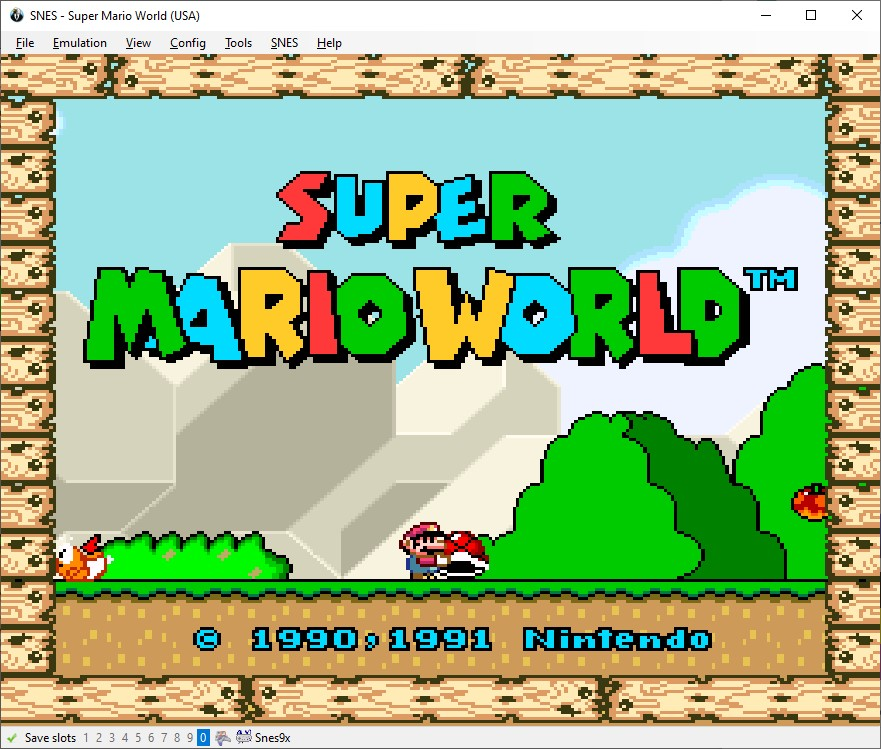
\includegraphics[width=0.75\textwidth]{start-screen}
    \caption{Screenshot of the Super Mario World start screen.}
    \label{fig:smw}
\end{figure}

The goal of this work is to train an AI to play the game using reinforcement learning.
For this task we use OpenAI Gym\footnote{\url{https://github.com/openai/gym}}---a library for developing and comparing reinforcement learning algorithms---and Gym Retro\footnote{\url{https://github.com/openai/retro}}---game integrations for Gym, including Super Mario World.

The aim is to make the agent learn and deal with the obstacles presented in the game.
Obstacles can consist of obstacles or enemies that must be defeated or dodged.
Look at how the agent learns to deal with obstacles presented by the game.
Test the agent on new/unseen data (in the form of levels the agent hasn't trained on).


\section{Reinforcement Learning} \label{s:reinforcement-learning}
Reinforcement learning (RL) is an area of machine learning which studies how intelligent agents learn to take actions in an environment by trial and error.
An agent is not told which actions to take, but must explore for itself which actions result in the highest reward.
The general idea behind RL is that rewarding good behavior or penalizing bad behavior makes the agent more or less likely to repeat this behavior in the future.
How the agent interacts with its environment is shown in the agent-environment loop in Figure \ref{fig:loop}.

\begin{figure}[htbp]
    \centering
    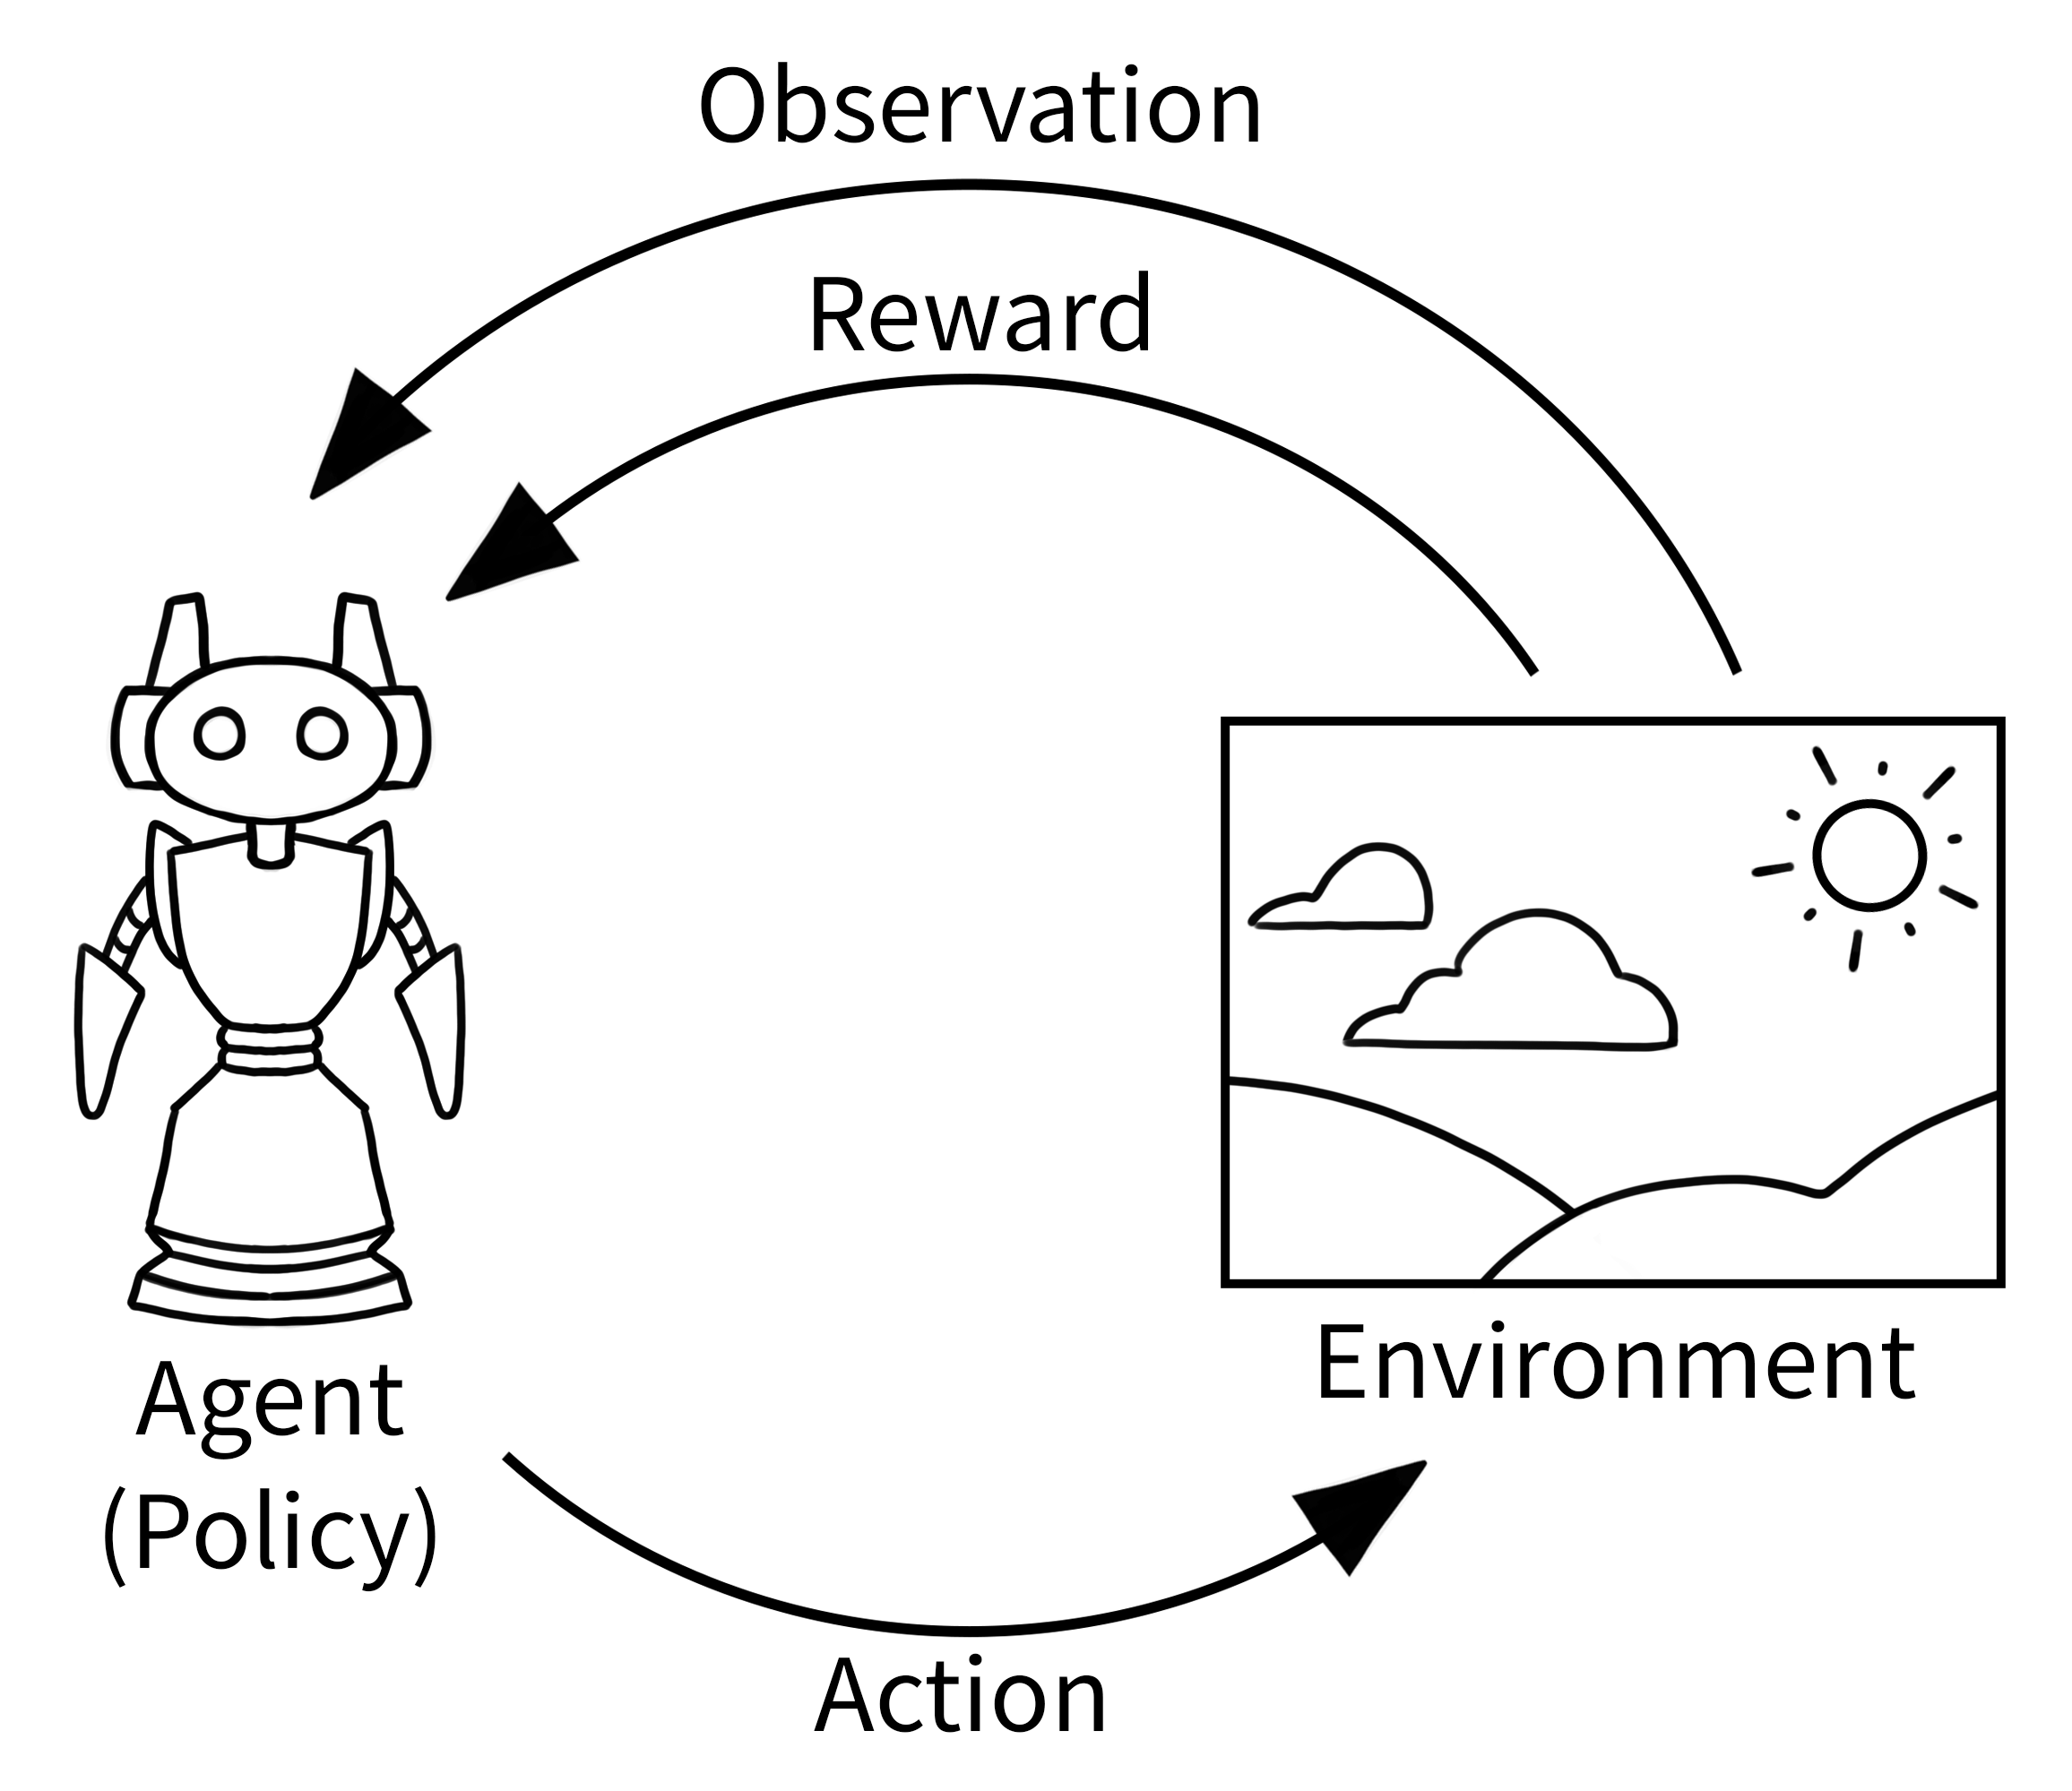
\includegraphics[width=0.6\textwidth]{AE_loop}
    \caption{The agent-environment interaction loop. Image source: \url{https://www.gymlibrary.dev}.}
    \label{fig:loop}
\end{figure}

The agent is trained in episodes which consist of a number of steps.
At each step, the agent receives the current observation and reward.
It then chooses an action to perform on the environment.
The action changes the state of the environment, and the environment returns a new observation and a reward based on how the action influenced the state.
Each component of the agent-environment interaction is described in more detail below.
\begin{description}[leftmargin=0cm]
    \item[Agent.]
    The decision maker of the process.
    How the agent chooses its actions is decided by a policy that tries to maximize the some form of cumulative reward.
    In our case the agent controls Mario and decides which actions he will take.
    \item[Action.]
    Agents interact with their environment through actions.
    In this game, an action is a combination of button presses.
    The set of all valid actions in an environment is called the \emph{action space}.
    \item[Environment.]
    World that the agent lives in (level of the game).
    The environment is represented by states, which are complete descriptions of the world.
    \item[Observation.]
    Part of the state that the agent is able to see (i.e., its immediate surroundings).
    Observations are, in this case, ``frames'' of the game.
    A frame is an image of the game; a raster of pixels of the form height\texttimes{}width\texttimes{}channel.
    The \emph{observation space} defines the structure and legitimate values an observation can take.
    \item[Reward.]
    A numeric value that describes how good (or bad) the result of an action is on the state of the environment.
    The value is determined by the reward function (more on rewards in Section \ref{s:reward}).
\end{description}

\section{Preprocessing} \label{s:preprocessing}
Before we can train our agent a number of preprocessing steps are necessary.
This includes a transformation of both the action and observation space.
Most of these steps are based on papers discussing the Arcade Learning Environment (ALE) \cite{bellemare2013arcade,machado2018revisiting}.
The ALE is a framework that allows people to develop AI agents for Atari\footnote{Atari 2600, originally known as Atari VCS (Video Computer System)} games and is commonly used to benchmark reinforcement learning algorithms.
Even though the ALE was created for Atari games, most of the preprocessing steps used are also applicable to the SNES (and Super Mario World).

\subsection{Action Space}
By default, the Gym Retro environment for Super Mario World uses a MultiBinary\footnote{\url{https://www.gymlibrary.dev/content/spaces/\#multibinary}} space with 12 elements (buttons).
Each action contains a value for every button in the action space where 0 (not pressed) or 1 (pressed). This results in $2^{12}=4096$ possible combinations.
Sticking to the default MultiBinary action space leads to three issues:
\begin{itemize}
    \item \textbf{Large action space.}
        Exploration in RL relies on some form of random sampling.
        If the action space is large, it will take longer for the agent to find good actions during exploration.
    \item \textbf{Invalid combinations.}
        Some combinations of buttons cannot be pressed at the same time (e.g. left and right arrows).
    \item \textbf{Irrelevant buttons.} Some buttons are only used to control the game menu or pause the game and have no effect on the actual gameplay.
\end{itemize}
To solve these problems we take a look at the SNES controller in Figure \ref{fig:snes-controller}.
The game was designed to be played on this controller, so the buttons used in Gym Retro correspond to the buttons on this controller.
Select, start, and the buttons on the back of the controller are not relevant for our agent.
The remaining buttons can be split into two clusters, arrow keys and special keys.
For each cluster, only one button can be pressed at any given time.
This translates to a MultiDiscrete\footnote{\url{https://www.gymlibrary.dev/content/spaces/\#multidiscrete}} action space, which is the cartesian product of (in this case two) discrete spaces.
The actions of both discrete spaces are described below.
In this game the \img{SuperNintendo-Button-X} and \img{SuperNintendo-Button-Y} keys serve the same function, so we only need to include one of them.
Not pressing a button is also a valid action.
\begin{itemize}
    \item \textbf{Arrow keys.} none, left (\img{SuperNintendo-Dpad-Left}), right (\img{SuperNintendo-Dpad-Right}), up (\img{SuperNintendo-Dpad-Up}), down (\img{SuperNintendo-Dpad-Down})
    \item \textbf{Special keys.} none, spin (\img{SuperNintendo-Button-A}), jump (\img{SuperNintendo-Button-B}), run/throw (\img{SuperNintendo-Button-X})
\end{itemize}
\begin{figure}[htbp]
    \centering
    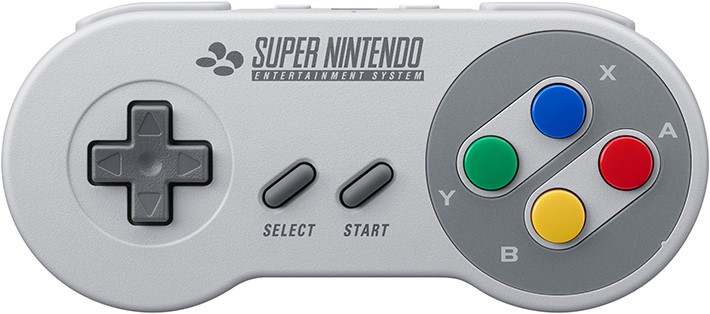
\includegraphics[width=.7\textwidth]{snes-controller}
    \caption{SNES controller.}
    \label{fig:snes-controller}
\end{figure}
The resulting MultiDiscrete action space contains $5\cdot4 = 20$ different actions.
So we have reduced the action space by a significant amount while maintaining the necessary actions to play the game.

\subsection{Observation Space}
\subsubsection{Transform observation}
To reduce the memory requirement, each observation is resized to 84\texttimes{}84 pixels.
The color is also converted to grayscale.
Figure \ref{fig:transformation} shows the result of this transformation.
Lowering the memory requirement significantly reduces the training time of the agent.
\begin{figure}[htbp]
    \centering
    \begin{subfigure}{.5\textwidth}
        \centering
        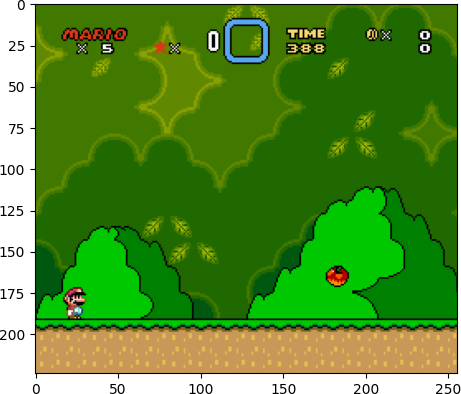
\includegraphics[height=6.35cm]{original_crop}
        \caption{Original}
        \label{fig:transformation:sub1}
    \end{subfigure}%
    \begin{subfigure}{.5\textwidth}
        \centering
        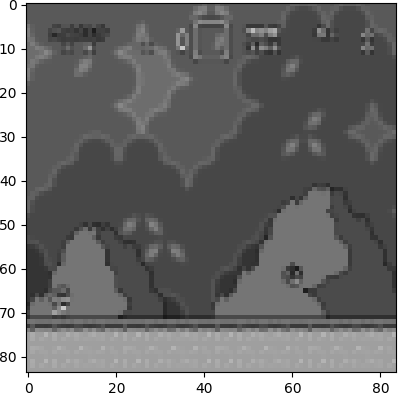
\includegraphics[height=6.35cm]{grayscale_crop}
        \caption{Transformed}
        \label{fig:transformation:sub2}
    \end{subfigure}
    \caption{Pixel Transformation.}
    \label{fig:transformation}
\end{figure}

\subsubsection{Skip frames}
SNES games run at 60 FPS (frames per second), which means there is very little change from frame to frame.
As such, it is unnecessary to input an action each frame (also human players do not press 60 buttons each second).
To create the effect of ``skipping'' frames we repeat each action over four frames and sum the accumulated rewards.
This can be seen as the equivalent of a human player holding the button for a few frames.
This change brings the agent closer to human behaviour and as an additional bonus speeds up the training of the agent.

\subsubsection{Stack frames}
The agent is trained on pixels, so each observation can be seen as some sort of screenshot of the game state.
By using a single frame, the agent cannot perceive the direction or velocity of movement (Is Mario going up or down? How fast is Mario moving?).
To solve this we ``stack'' four subsequent observations on top of each other and use the resulting observation for training.
Each observation is placed in a queue and concatenated with the previous three most recent observations.
On Figure \ref{fig:stack} we can see based on the last four observations that Mario is jumping to the right.
\begin{figure}[htbp]
    \centering
    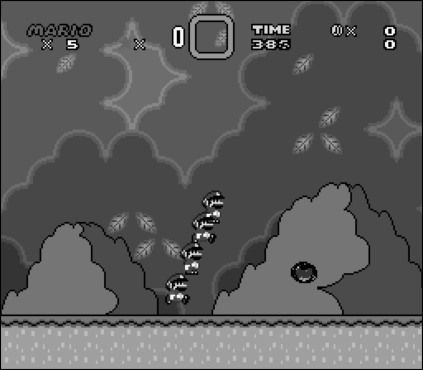
\includegraphics[height=6cm]{stacked}
    \caption{Stacking four subsequent observations.}
    \label{fig:stack}
\end{figure}

\subsection{Other}
\subsubsection{Episodic Life}
In Gym environments, the current episode ends when the ``done'' signal is received.
However, in this game the player starts with five lives, so this signal is only sent once the life counter reaches zero.
Every time Mario dies the game exits the current level and returns to the menu.
Since no signal has been sent, the agent does not understand it is no longer in the intended level, and as a result can get stuck in the game menu or even enter another level by accident.
To avoid this we want to terminate the episode after a single life is lost.
Ending the episode after a life is lost also creates a positive side effect; the longer the episode continues, the more rewards the agent can gain, so the agent learns to avoid death without explicitly defining a penalty for losing a life.

\subsubsection{Sticky Actions}
Super Mario World is deterministic. 
Enemies and other moving objects will always appear in the same location at the same timestamp of a level.
We want the AI to learn a policy that will work on other levels, not just memorize one action sequence in a single level, so we need to introduce some form of stochasticity.
With ``sticky actions'' \cite{machado2018revisiting} each time the agent chooses a new action there is a 25\% chance it will repeat the previous action instead.
This makes it so the agent is never sure where it will end up at any given time, and forces it to act accordingly.

\section{Reward} \label{s:reward}
The goal of an agent in reinforcement learning is to maximize its cumulative reward.
After each step the agent receives a reward from the environment, which describes how good (or bad) the action taken during this step was.
The value of this reward is determined by the reward function.
A well designed reward function is important in order for the agent to achieve the desired behavior.

Gym Retro's default rewards are most often tied to the game score.
In Super Mario World the player gains points by collecting coins or defeating enemies.
However, the goal of a human player is usually beating the game by completing all the different levels, not maximizing the score.
When trained using the score as reward, the agent will find some unintended way to maximize its score (defeating the same enemy over and over, for example) without ever finishing a level.
An alternative reward is needed if we want the agent to act similar to human players.

In theory you could design a reward function that gives $+1$ for completing a level of the game.
This reward is not practical though, because it is too ``sparse''.
The duration of a single episode is limited to several thousand steps due to the timer present in the game.
It is very unlikely the agent will reach the end of a level by taking random actions before the timer expires, so it might never see a positive reward.
The agent cannot learn which actions are good with such a restrictive reward.
So we are looking for some reward that is easier to obtain but should still result in completing a level if maximized.

Mario starts each level on the left side and the flag which indicates the end of that level is always on the right side.
We can reward the agent for moving right by comparing Mario's horizontal position (x-value) before and after each step.
Subtracting the x-value $x_{t}$ at step $t$ with that of the previous step $x_{t-1}$ can result in the following three scenarios.
\begin{eqnarray*}
    x_{t} - x_{t-1} > 0&\iff&\text{Mario is moving to the right}\\
    x_{t} - x_{t-1} = 0&\iff&\text{Mario is standing in place}\\
    x_{t} - x_{t-1} < 0&\iff&\text{Mario is moving to the left}
\end{eqnarray*}
The magnitude of the reward is determined by how much Mario moved in a single step.
Moving faster will result in a larger reward (or penalty in case of moving left).

There is one more simple improvement we can make.
By applying a small penalty ($-1$) on each step we incentivize the agent to try to complete the level as fast as possible.
Combining both gives us the reward $r_{t}$ at each step $t$.
\[r_{t} = x_{t} - x_{t-1} - 1\]


\section{Algorithm} \label{s:algorithm}
With the preprocessing and reward design completed, only the choice of algorithm remains before we can start training.
Reinforcement learning algorithms can be divided into two branches: \emph{Model-Based RL} and \emph{Model-Free RL}.
In model-based RL the agent uses predictions of the environment response.
This allows the agent to plan ahead, seeing what would happen for a range of possible actions.
The main benefit of model-based algrithms is sample efficiency.
The downside is that a ground-truth model of the environment is usually not available
In contrast, model-free algorithms sample purely from experience and never use generated predictions of the next state/reward.
This makes them easier to implement and tune but also less sample efficient.
In the case of Super Mario World, we opt for a model-free algorithm.

In model-free RL there are two main approaches to training agents: \emph{Q-Learning} and \emph{Policy Optimization}.
Q-learning methods learn an approximator for the optimal action-value function.
In general, Q-learning methods are more sample efficient because they can reuse old data more effectively, while policy optimization methods are more stable and reliable.

Proximal Policy Optimization (PPO) \cite{schulman2017proximal} is a state-of-the-art policy optimization algorithm.
PPO is motivated by the question: ``How can we take the biggest possible improvement step on a policy using the data we currently have, without stepping so far that we accidentally cause performance collapse?''
PPO-clip (the most common variant of PPO, also the variant implemented in the Stable Baselines library\footnote{\url{https://github.com/DLR-RM/stable-baselines3}}) achieves this with clipping in the objective function to remove incentives for the new policy to get far from the old policy.

PPO trains a stochastic policy in an on-policy way.
This means that it explores by sampling actions according to the latest version of its stochastic policy.
The amount of randomness in action selection depends on both initial conditions and the training procedure.
Over the course of training, the policy typically becomes progressively less random, as the update rule encourages it to exploit rewards that it has already found.

\subsection{Hyperparameters}
The following hyperparameters for PPO were used to train the agent.
Unmentioned parameters use the default value defined in the Stable Baselines library.
\begin{table}[htbp]
\centering
\begin{tabularx}{\linewidth}{llX}
\toprule
Hyperparameter & Value & Description \tabularnewline
\midrule
Learning rate & \num{1e-4} & Step size of the Adam optimizer. \tabularnewline
Horizon (T) & 512 & Number of steps to run for each environment per update. Rollout buffer size is equal to horizon $\times$ environments. \tabularnewline
Num. environments & 8 & Number of environments running in parallel. \tabularnewline
Minibatch size & 512 & Steps of interaction for the agent and the environment in each epoch. \tabularnewline
Num. epochs & 2 & Number of epochs of interaction to perform. \tabularnewline
Clipping range ($\epsilon$) & 0.1 & Hyperparameter for clipping in the policy objective. \tabularnewline
Entropy coeff. ($c_1$) & 0.001 & Helps prevent premature convergence of one action probability dominating the policy and preventing exploration \tabularnewline
\bottomrule
\end{tabularx}
\caption{PPO hyperparameters.}
\label{table:hyperparams}
\end{table}

\section{Training \& Results} \label{s:training-results}
\subsection{Model A}
Trained for 25 million time steps on the level 'YoshiIsland1'.
Most basic level (avoid enemies, jump over pit).
\begin{figure}[htbp]
    \centering
    \begin{subfigure}{.5\textwidth}
        \centering
        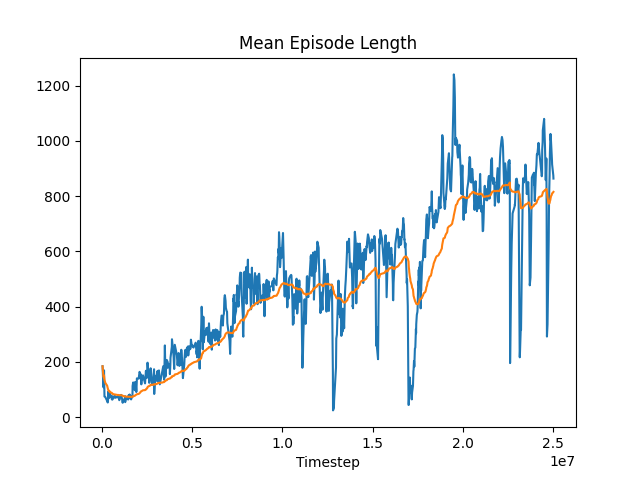
\includegraphics[width=\textwidth]{PPO_YoshiIsland1_len}
        \label{fig:result1:sub1}
    \end{subfigure}%
    \begin{subfigure}{.5\textwidth}
        \centering
        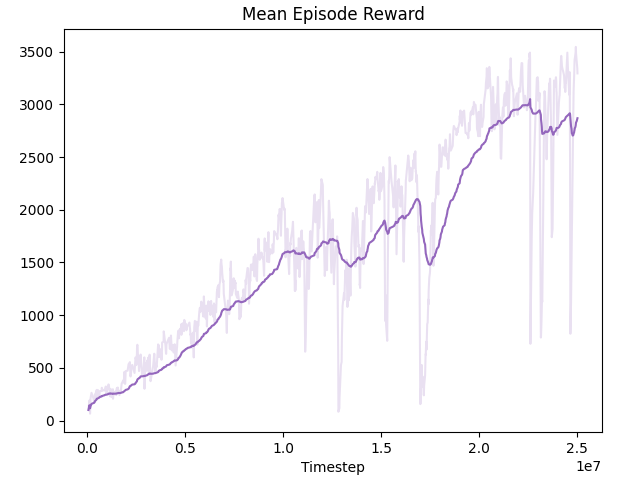
\includegraphics[width=\textwidth]{PPO_YoshiIsland1_rew}
        \label{fig:result1:sub2}
    \end{subfigure}
    \caption{Training results PPO YoshiIsland1.}
    \label{fig:result1}
\end{figure}

\subsection{Model B}
\begin{figure}[htbp]
    \centering
    \begin{subfigure}{.5\textwidth}
        \centering
        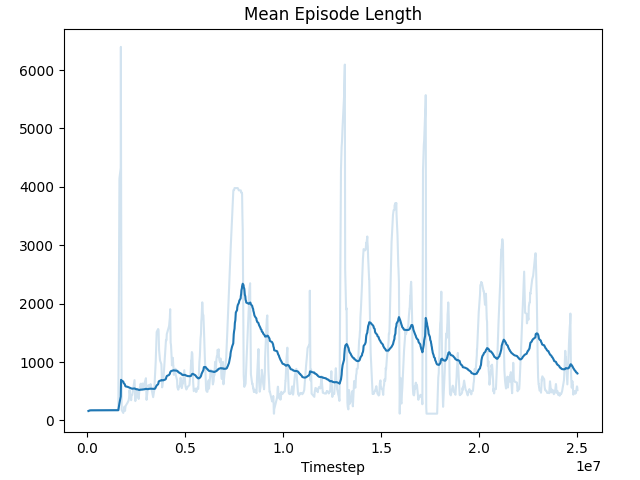
\includegraphics[width=\textwidth]{PPO_YoshiIsland2_len}
        \label{fig:result2:sub1}
    \end{subfigure}%
    \begin{subfigure}{.5\textwidth}
        \centering
        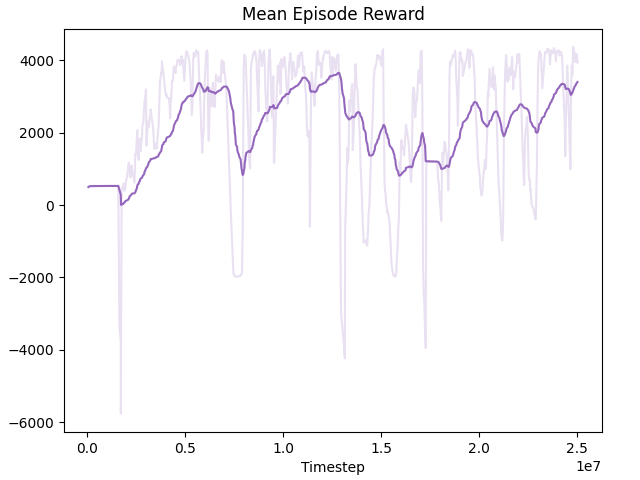
\includegraphics[width=\textwidth]{PPO_YoshiIsland2_rew}
        \label{fig:result2:sub2}
    \end{subfigure}
    \caption{Training results PPO YoshiIsland2.}
    \label{fig:result2}
\end{figure}

\printbibliography
\end{document}